
\subsection{Clustering}
Clustering is a fundamental technique used to group similar data points based on their characteristics. It is particularly useful in sensor data analysis for automotive applications, enabling the effective detection and tracking of objects such as vehicles, obstacles, and pedestrians.
\par
Among various clustering algorithms available, DBSCAN (Density-Based Spatial Clustering of Applications with Noise) stands out due to its ability to automatically detect clusters of varying shapes and sizes (see \cite{geeksforgeeks_dbscan}), and to effectively identify and manage noise or outliers. Unlike centroid-based methods such as K-means, which require specifying the number of clusters in advance and struggle with irregularly shaped data, DBSCAN identifies clusters based on the density distribution of data points. Additionally, hierarchical methods like agglomerative clustering, although flexible, tend to be sensitive to noise and computationally expensive for large datasets.

\begin{table}[htbp]
\centering
\resizebox{\columnwidth}{!}{%
\begin{tabular}{|l|l|p{3.5cm}|p{3.5cm}|p{3.5cm}|}
\hline
\textbf{Algorithm} & \textbf{Type} & \textbf{Strengths} & \textbf{Weaknesses} & \textbf{Best Use Case} \\ \hline
DBSCAN & Density-Based & \begin{itemize}
    \item Automatically detects clusters of \textbf{different shapes and sizes}
    \item Identifies \textbf{outliers (noise points)}
\end{itemize} & \begin{itemize}
    \item Computationally expensive for \textbf{large datasets}
\end{itemize} & Radar object detection with noise filtering \\ \hline
K-Means & Centroid-Based & \begin{itemize}
    \item Fast and efficient for \textbf{large datasets}
\end{itemize} & \begin{itemize}
    \item Requires a \textbf{fixed number of clusters (K)}
    \item Struggles with \textbf{irregularly shaped clusters}
\end{itemize} & Segmenting structured radar data with known object counts \\ \hline
Agglomerative & Hierarchical & \begin{itemize}
    \item Does not require specifying number of clusters
    \item Can be modified to detect \textbf{hierarchical structures}
\end{itemize} & \begin{itemize}
    \item Can be \textbf{sensitive to noise}
    \item Computationally expensive for \textbf{large datasets}
\end{itemize} & Grouping similar radar signatures in post-processing \\ \hline
\end{tabular}%
}
\caption{Comparison of Clustering Algorithms}
\label{tab:clustering_algorithms}
\end{table}

For this project, DBSCAN's strengths align closely with the requirements of radar object detection, where the number of detected objects can change dynamically and the presence of noise is common. DBSCAN's capability to handle varying densities and noisy data makes it the optimal choice for accurately and efficiently analyzing real-time radar sensor data in automotive applications.

However, this is insufficient to fully meet the requirements of object detection. It is acknowledged that DBSCAN is among the most efficacious and straightforward instruments available for achieving this objective. However, it is important to note that the sizes of the objects under observation can vary significantly from one frame to the next, and the presence of noise can introduce additional variability. To address these challenges, a two-stage clustering approach was chosen, utilizing DBSCAN as a filter and a clustering algorithm.
The first stage that acts as a filter with DBSCAN parameterized by an Epsilon of \SI{2}{\meter} and a minimum number of samples to specify a core point of 2.
The justification for using it as a filter is that, at first, a broad or permissive set of parameters is applied, making it easier to filter out points or data that are considered as noise. This is not due to the presence of "real" noise; rather, it is owing to a lack of the required amount of points to qualify as an object.
This principle is represented in the next figure:
\begin{figure}[!htbp]
    \centering
    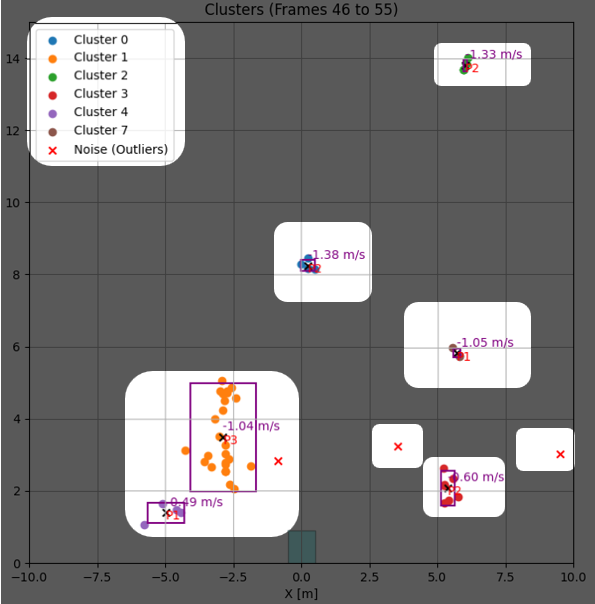
\includegraphics[width=1.0\linewidth]{images/clustering.png}
    \caption{First clustering stage}
    \label{fig: First clustering stage}
\end{figure}
\FloatBarrier\noindent
It can be seen that there are three points that are not included in the clusters and seem to be outliers.
These points might belong to an object, but most likely they are caused by clutter or noise.
As they are not included in clusters after first stage, they are discarded and only the points that are included in clusters are passed to the second stage.
\par
The second stage utilizes DBSCAN with a finer set of parameters.
In this stage, Epsilon was chosen to be equal to \SI{1}{\meter} and the minimum number of samples to specify a core point was set to 4.
This results in finer clusters, preventing objects which are close to each other to be recognized as one single cluster.
The clusters are then passed to the brake controller for final object detection and handling of approaching targets.